% ─────────────────────────────────────────────────────────────────────────────
%  Progress Report — Habib University CS Algorithms Project
%  ACL two-column, A4, 2 pages
%  Overleaf: upload this file + upload results_combined.png into a figures/ folder
% ─────────────────────────────────────────────────────────────────────────────
\documentclass[11pt,twocolumn,a4paper]{article}

\usepackage[utf8]{inputenc}
\usepackage[T1]{fontenc}
\usepackage{times}
\linespread{1.05}
\usepackage{microtype}
\usepackage{xcolor}
\usepackage{graphicx}
\graphicspath{{figures/}}
\usepackage{booktabs}
\usepackage{enumitem}
\usepackage[top=0.75in, bottom=0.75in, left=0.80in, right=0.80in]{geometry}
\usepackage[
  colorlinks=true,
  linkcolor=blue!50!black,
  citecolor=blue!50!black,
  urlcolor=blue!50!black
]{hyperref}
\usepackage{caption}

\captionsetup{font=small, labelfont=bf, skip=5pt}
\setlength{\parskip}{5pt}
\setlength{\parindent}{10pt}
\setlength{\intextsep}{7pt}
\setlength{\textfloatsep}{8pt}
\setlength{\abovecaptionskip}{4pt}
\setlength{\belowcaptionskip}{0pt}

\setlist[itemize]{itemsep=3pt, topsep=4pt, leftmargin=14pt}
\setlist[enumerate]{itemsep=3pt, topsep=4pt, leftmargin=16pt}

% compact section headings
\makeatletter
\renewcommand\section{\@startsection{section}{1}{\z@}%
  {-10pt \@plus -2pt \@minus -2pt}%
  {6pt \@plus 2pt}%
  {\normalfont\large\bfseries}}
\makeatother

% ─────────────────────────────────────────────────────────────────────────────
\title{\vspace{-1.6em}%
\textbf{Progress Report: Comparing Shortest-Path Algorithms on 4-Connected Grid Maps}\\[-2pt]
{\normalsize Dijkstra, A*, and Jump Point Search (JPS4)}\vspace{-0.4em}}

\author{%
  Jazib Waqas \enspace Salman Adnan \enspace Hunain Abbas \\[-1pt]
  {\small jw08048 \textperiodcentered\ sa07885 \textperiodcentered\ sh08466}%
  \vspace{-0.8em}}
\date{}

% ─────────────────────────────────────────────────────────────────────────────
\begin{document}
\maketitle

\begin{abstract}
\vspace{-4pt}
This report describes our progress on comparing three pathfinding algorithms
(Dijkstra, A*, and Jump Point Search for 4-connected grids, or JPS4) on grid
maps with randomly placed obstacles. We measure how many cells each algorithm
visits and how long it takes across three obstacle densities. So far, A* cuts
Dijkstra's node count roughly in half, which was more or less expected; JPS4
reduces it further at low densities by skipping over open space entirely,
though it does not hold up as well once obstacles get denser, which was
a bit surprising. We have a working benchmark, preliminary results, and a
Snake-game visualization in development to demonstrate all three algorithms
side by side.
\end{abstract}

% ── 1. Problem ───────────────────────────────────────────────────────────────
\section{Problem}

Grid-based pathfinding comes up in a lot of areas like video games, robotics,
and logistics, and it is easy to underestimate how much work a naive search
actually does. In a \emph{4-connected grid}, each cell connects to its four
cardinal neighbours (up, down, left, right) at unit cost, and blocked cells
act as walls. The task is: given a start cell and a goal cell, find the
shortest path between them.

A naive search checks every reachable cell before it can confirm the path is
optimal. On large maps this is too slow. Smarter algorithms cut this down in
two ways: \textbf{heuristics} bias the search toward the goal to avoid wasting
effort in the wrong direction, while \textbf{symmetry pruning} skips over empty
regions where there is nothing useful to find.

We evaluate each algorithm on two metrics: \textbf{node expansions} (how many
cells were processed, independent of hardware) and \textbf{search time in ms}
(wall-clock time, which also reflects implementation cost).

% ── 2. Algorithms ────────────────────────────────────────────────────────────
\section{Algorithms}

\textbf{Dijkstra} is the baseline. It expands cells in order of increasing
distance from the start, processing every cell at cost $d$ before any at cost
$d{+}1$. It always returns the shortest path but has no directional sense,
searching equally in all directions regardless of where the goal is. Because it
does not know where the goal is, it essentially maps the entire reachable area
before it can confirm the shortest path.

\textbf{A*} adds a heuristic: at each step it picks the cell with the lowest
estimated total cost (current cost plus Manhattan distance to the goal). This
directs the search toward the goal rather than spreading outward uniformly
\cite{hart1968}. On uniform-cost 4-connected grids the Manhattan distance is a
valid lower bound on remaining cost, so A* still guarantees an optimal path.

\textbf{JPS4} builds on A* but adds symmetry pruning \cite{harabor2011,
baum2025}. When moving in a straight line through open space, every intermediate
cell produces identical cost and identical neighbour options, so visiting each
one adds no information. JPS4 skips those cells and stops only at \emph{jump
points}: places where an obstacle forces a meaningful routing choice. Only jump
points enter the open list, keeping it significantly smaller. The 4-connected
(cardinal-only) case studied by Baum \cite{baum2025} is harder than the original
8-connected formulation because the absence of diagonal moves changes where
symmetric paths arise and requires different pruning rules.

We set things up so that all three algorithms run through the same search loop,
with the heuristic and successor function swapped in per algorithm. That way
any difference we measure is actually from the algorithm itself, not from
one implementation being written more carefully than another.

% ── 3. Preliminary Results ───────────────────────────────────────────────────
\section{Preliminary Results}

We generated 50$\times$50 grids with random obstacles at three densities (15\%,
28\%, and 40\% blocked). Start and goal were placed as far apart as possible and
confirmed reachable. All three algorithms ran on the same grid; a trial was
counted only if all three returned a valid path. We ran 24 trials per density
with seed 42.

\begin{table}[h]
\centering
\small
\setlength{\tabcolsep}{3.8pt}
\begin{tabular}{l rr rr rr}
\toprule
  & \multicolumn{2}{c}{15\% blocked}
  & \multicolumn{2}{c}{28\% blocked}
  & \multicolumn{2}{c}{40\% blocked} \\
\cmidrule(lr){2-3}\cmidrule(lr){4-5}\cmidrule(lr){6-7}
  & Exp. & ms & Exp. & ms & Exp. & ms \\
\midrule
Dijkstra  & 2062 & 7.07 & 1659 & 4.96 & 915 & 2.73 \\
A*        & 1020 & 3.74 &  629 & 2.11 & 513 & 1.70 \\
JPS4      &  488 & 4.43 &  970 & 6.22 & 682 & 3.13 \\
\bottomrule
\end{tabular}
\caption{Mean node expansions and search time per density (24 trials, 50$\times$50 grid).}
\label{tab:prelim}
\end{table}

\begin{figure}[h]
\centering
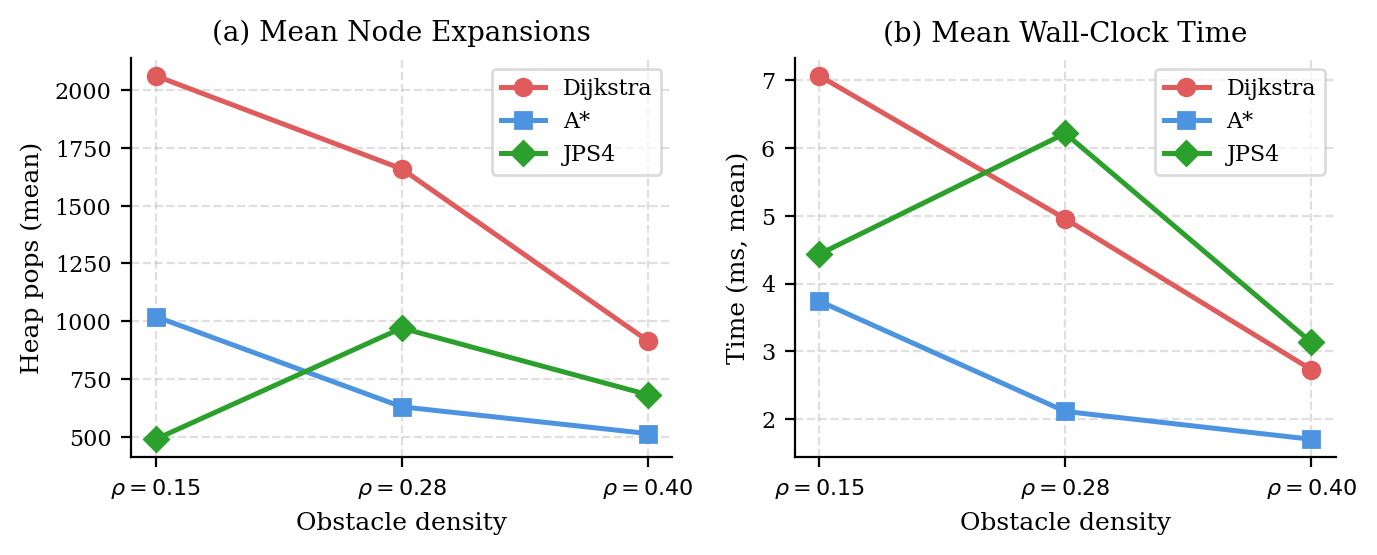
\includegraphics[width=0.96\columnwidth]{results_combined.png}
\caption{Mean expansions (left) and search time in ms (right) vs.\ obstacle density.}
\label{fig:results}
\end{figure}

At 15\% density, JPS4 visits only 488 nodes versus 1020 for A* and 2062 for
Dijkstra, a 76\% reduction over Dijkstra. Open maps give JPS4 long unobstructed
corridors to jump through, so the pruning is highly effective.

At 28\% density, JPS4's count rises to 970, which is actually above A*'s 629
which was not what we initially expected. Denser obstacles shorten corridors, so
each jump covers less ground while the per-step cost of checking for forced
neighbours stays the same. The pruning still happens, it just stops being
worth it.

On wall-clock time, JPS4 is slower than A* at all densities despite visiting
fewer nodes at low density. JPS4's inner loop is more complex than A*'s simple
four-way neighbour lookup, and Python's interpreter amplifies this per-step cost.
In compiled implementations (C++, Java) this overhead is negligible
\cite{harabor2011}. All three algorithms returned equal path lengths on every
trial, which confirms that all three implementations are correct.

For now, node expansions are the more reliable number to look at. The timing
results should become clearer once we test on larger grids where the
differences are big enough to matter; we are still working out how to
get a cleaner read on the inner loop cost.

% ── 4. Challenges Identified ─────────────────────────────────────────────────
\section{Challenges Identified}

\begin{enumerate}
  \item \textbf{Fair timing.} Python is noticeably harder on JPS4 than on
    the simpler A* loop, which makes the wall-clock numbers hard to interpret.
    Node expansions give a cleaner picture of what is actually happening
    algorithmically. We are planning to look more carefully at where the time
    is going inside the jump function.

  \item \textbf{Grid scale.} Everything finishes in under 10ms on a
    50$\times$50 grid, so the timing gaps are too noisy to say much about.
    The node expansion counts are meaningful but we really need larger maps
    to see a convincing difference. We think JPS4's advantage should grow
    on 100$\times$100 and 200$\times$200 since longer open corridors give
    it more room to skip.

  \item \textbf{Density boundary.} JPS4 clearly wins at low density but
    falls behind A* somewhere between 15\% and 28\% and we have not
    pinned down where exactly yet. Finding that cross-over is actually one
    of the more interesting things left to do, since it tells you under
    what conditions JPS4 is worth the extra overhead.
\end{enumerate}

% ── 5. Next Plan ─────────────────────────────────────────────────────────────
\section{Next Plan}

\begin{itemize}
  \item \textbf{Week 13:} Scale the benchmarks up to 100$\times$100 and
    200$\times$200. We also want to sweep density more finely (5\% to 50\%
    in 5\% steps) to find where A* and JPS4 actually cross over, since
    that is the main open question coming out of the preliminary run.

  \item \textbf{Week 13:} Finish the Snake-game visualization. The game
    runs all three algorithms already but the compare mode still needs
    work, and the goal is to show each algorithm's route in a distinct
    color so the behavioral difference is visible in real time.

  \item \textbf{Week 14:} Put together the final tables and figures once
    the larger-grid data is in. Write up the discussion, mainly around
    how our numbers compare to what Baum (2025) reports.

  \item \textbf{Week 15:} Prepare the presentation and do a run-through
    of the live demo before submitting.
\end{itemize}

% ── References ───────────────────────────────────────────────────────────────
\begin{thebibliography}{9}

\bibitem{baum2025}
M.~Baum.
\newblock Jump point search pathfinding in 4-connected grids.
\newblock \emph{arXiv:2501.14816}, 2025.
\newblock \href{https://arxiv.org/abs/2501.14816}{\texttt{arxiv.org/abs/2501.14816}}

\bibitem{hart1968}
P.~E.~Hart, N.~J.~Nilsson, and B.~Raphael.
\newblock A formal basis for the heuristic determination of minimum cost paths.
\newblock \emph{IEEE Trans.\ Syst.\ Sci.\ Cybern.}, 4(2):100--107, 1968.
\newblock \href{https://doi.org/10.1109/TSSC.1968.300136}{\texttt{doi:10.1109/TSSC.1968.300136}}

\bibitem{harabor2011}
D.~Harabor and A.~Grastien.
\newblock Online graph pruning for pathfinding on grid maps.
\newblock In \emph{AAAI-11}, pages 1114--1119, 2011.
\newblock \href{https://ojs.aaai.org/index.php/AAAI/article/view/7994}{\texttt{ojs.aaai.org $\cdot$ article/7994}}

\end{thebibliography}

\end{document}
